\section{Institutional Background: The 2021 Privacy Regime}
\label{sec:institution}

\subsection{Apple App Tracking Transparency}

Apple announced ATT at its Worldwide Developers Conference in June 2020. The policy took effect with the release of iOS 14.5 on 26 April 2021. Under ATT, an app must obtain explicit user permission before tracking a user across other companies' apps and websites or accessing the advertising identifier. If a user declines, the app receives a zeroed identifier and cannot conduct user-level attribution, retargeting, or lookalike-audience construction across apps \cite{apple2020}. ATT therefore changed the default rules of the mobile advertising market: cross-app tracking moved from opt-out to opt-in.

The economic consequences of ATT have been documented in several markets. ATT reduced advertising effectiveness and sales for e-commerce firms \cite{aridor2024}. It lowered app monetization for developers \cite{kesler2023}. It also changed competition and entry in the app ecosystem \cite{cheyre2024}. These findings establish that ATT is a substantive shock to the third-party data ecosystem, not a narrow technical change.

\subsection{China's Personal Information Protection Law}

China's PIPL was adopted on 20 August 2021 and took effect on 1 November 2021. The law establishes a legal basis for processing personal information, requires informed consent for sensitive information and cross-border transfers, and imposes minimization and accountability obligations on data controllers \cite{pipl2021}. The Data Security Law, effective 1 September 2021, introduced data classification and security assessment rules for important data and cross-border data flows \cite{dsl2021}. Together, the two laws raised the cost of acquiring, sharing, and using third-party personal data.

For Chinese digital firms, the 2021 regime is a combined shock. ATT cut the default supply of cross-app identifiers on Apple devices. PIPL and the Data Security Law raised the legal and compliance cost of using personal data on all devices. The two shocks are adjacent in time and complementary in mechanism. We therefore define 2021Q3 as the first post-shock quarter: ATT had taken effect at the end of Q2, and firms began adjusting their data, advertising, and compliance practices in Q3. Figure \ref{fig:timeline} summarizes the timeline.

\subsection{Why 2021 Is a Useful Shock}

The 2021 regime has three features that make it useful for identification. First, the timing was set by Apple and by the Chinese legislature, not by individual firms. A single A-share firm could not choose the implementation date or the content of the rules. Second, the shock changed the availability and cost of third-party data without directly changing firms' physical capital, labor, or product markets. Third, the shock had differential intensity: firms with different ex ante data architectures were exposed to different degrees. The identifying variation is therefore a common shock interacted with predetermined firm-level exposure.

The design does not isolate the effect of ATT from the effect of PIPL. Instead, it estimates the combined effect of the 2021 privacy regime on firms with different third-party data dependence. This is the relevant object for asset valuation: investors price the net effect of the regime, not the effect of a single statute. The next sections describe how we measure exposure and how we estimate its valuation effect.

\begin{figure}[htbp]
\centering
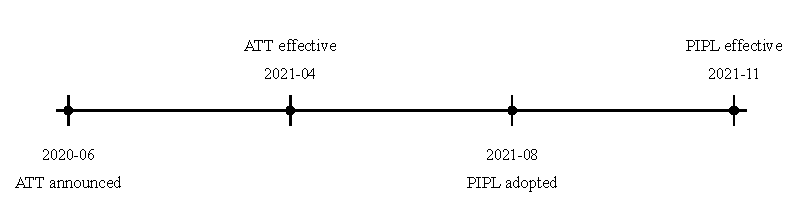
\includegraphics[width=0.95\textwidth]{fig1_timeline.pdf}
\caption{Timeline of the 2021 privacy regime. ATT was announced in June 2020 and took effect with iOS 14.5 in April 2021. PIPL was adopted in August 2021 and implemented in November 2021. The empirical analysis defines 2021Q3 as the first post-shock quarter.}
\label{fig:timeline}
\end{figure}
